\section{Experiments}
\subsection{Experiment Setting}
% \subsubsection{Training Data}
% To train \model effectively across diverse multimodal tasks, we curate a training dataset comprising three main sources: video-language instruction data, visual document retrieval, and image-based vision tasks.

% First, we utilize training data from LLaVA-Hound~\citep{llavahound}, which includes synthetic video-caption pairs and video QA examples generated by ChatGPT. Specifically, we use 300k video-caption pairs and 240k video QA pairs. For the caption data, we adopt two formats: using the caption as the query and video as the target in a video retrieval setup, or using the video as the query to retrieve the most relevant textual description from candidate captions.

% Second, for visual document retrieval tasks, we incorporate datasets from \texttt{ViDoRe}~\citep{colpali} and \texttt{VisRAG}~\citep{visrag}, including \texttt{colpali train set} (118k), \texttt{VisRAG synthetic} (239k), and \texttt{VisRAG in-domain} (123k), which provide training examples for image-based document understanding and retrieval.

% Finally, we include image-text datasets from MMEB-train~\citep{vlm2vec} to support generalization across a wide range of visual understanding tasks, including question answering, classification, retrieval, and visual grounding. These datasets help improve the robustness of the learned embeddings across multiple tasks.

% corrected alpha=32->64
\subsubsection{Training Setting}
We train \model using Qwen2-VL-2B-Instruct\footnote{\url{https://huggingface.co/Qwen/Qwen2-VL-2B-Instruct}}~\citep{qwen2vl} as backbone, a batch size of 1,024 for 2K steps and a homogeneous sub-batch size of 64, with the loss temperature set to 0.02. To support scalable training, we use GradCache~\citep{gradcache} to enable large global batch sizes and run all experiments on 8 H100 GPUs. For parameter-efficient training, we apply LoRA tuning with a rank of 16 and scaling factor $\alpha=64$ using the PEFT framework~\citep{peft}. We use 8 uniformly sampled frames to represent each video during both training and evaluation. 

Training \model with a 2B backbone on 8 NVIDIA H100 GPUs takes approximately 15 hours per 1k steps. Considering the training cost, all analyses in this work are conducted using the 2B backbone. Nevertheless, our framework is general and can be readily adapted to larger MLLMs, which may yield stronger embedding models.


% \semih{Is this correct? Are we not reporting other metrics? } Rui: good catch! visdoc uses ndcg@5.
% In our setting—where each query has a single correct answer—Recall@1 is equivalent to Precision@1 and Accuracy. Additional training details can be found in Appendix~\ref{app:train-detail}.

\subsubsection{Baselines}
% While effective for structured documents, ColPali is computationally expensive at inference time and does not generalize to other modalities. 
% For the video domain, we include InternVideo2-1B\footnote{OpenGVLab$/$InternVideo2-Stage2\_1B-224p-f4}~\citep{internvideo}, a model extensively trained on large-scale video data and considered state-of-the-art for video retrieval tasks.


We compare against several VLM embedding models, including GME~\citep{gme}, VLM2Vec~\citep{vlm2vec}, and LamRA~\citep{lamra}, most of which are primarily trained on image-text pairs. While these models are not explicitly designed for video tasks, many can be adapted to handle video inputs by encoding multiple frames as sequential images. For video evaluation, GME and LamRA use a single middle frame, while the remaining models use 8 uniformly sampled frames.
% However, technical limitations—such as input processing mismatches (e.g., reliance on specific chat-style templates), input format constraints (e.g., InternVideo2 only supports 4-frame inputs), or high memory usage (e.g., ColPali)—prevent some baselines from producing reliable results on certain datasets. 

In addition, to provide a fair comparison across modalities, we evaluate VLM2Vec-V2 against representative models specialized for each modality. Specifically, we include ColPali~\citep{colpali} (v1.3), a model tailored for document retrieval using a late interaction matching mechanism. 

\subsection{Evaluation Metrics}
We use Hit@1 as the primary evaluation metric for all video and image tasks, measuring the proportion of queries where the correct target is ranked at the top. For visual document tasks, we report NDCG@5 to remain consistent with prior work in this domain.


\subsection{Main Results}    
% \begin{table}[ht]
% \centering
% \caption{Performance comparison between baseline models and our {\model} across image, video, and visual document tasks. Here, CLS denotes classification, QA denotes question answering, RET denotes retrieval, GD denotes grounding, and MRET denotes moment retrieval.}
% \resizebox{\textwidth}{!}{
% \begin{tabular}{l|ccccc|ccccc|c}
% \toprule
%  & \multicolumn{5}{c|}{\textbf{MMEB-V1}} & \multicolumn{6}{c}{\textbf{MMEB-V2}} \\
% \textbf{Modality} & \multicolumn{5}{c|}{\textbf{Image}} & \multicolumn{5}{c|}{\textbf{Video}} & \textbf{VisDoc} \\
% % \cmidrule(lr){2-6} \cmidrule(lr){7-11} \cmidrule(lr){12-12}
%  & \textbf{CLS} & \textbf{QA} & \textbf{RET} & \textbf{GD} & \textbf{Overall} 
%  & \textbf{CLS} & \textbf{QA} & \textbf{RET} & \textbf{MRET} & \textbf{Overall} 
%  & \textbf{RET} \\
% \midrule
% \textbf{\# of Datasets} $\rightarrow$ & 10 & 10 & 12 & 12 & 36 & 5 & 4 & 5 & 3 & 17 & 6 \\
% \midrule
% \multicolumn{17}{c}{\textbf{Baseline Models}} \\ \midrule
% LamRA-7B        & 58.6 & 25.9 & 69.3 & 63.2 & 53.6 & 41.2 & -    & 24   & -    & -    & -    \\
% \rowcolor{gray!10}
% E5-V-8B           & 21.8 & 15.2 & 7.0  & 4.4  & 13.3 & 25.9 & 26.9 & 21.4 & 38.5 & 27.0 & -    \\
% GME-2B              & 55.7 & 47.4 & 33.7 & 29.4 & 52.7 & 36.6 & 37.7 & 26.1 & 31.0 & 32.9 & -    \\
% \rowcolor{gray!10}
% GME-7B              & 58.3 & 50.9 & 38.5 & 33.4 & 56.9 & -    & -    & -    & -    & -    & -    \\
% InternVideo2-1B     & -    & -    & -    & -    & -    & 55.7 & 38.7 & 40.8 & 12.6 & 41.4 & -    \\
% \rowcolor{gray!10}
% ColPali             & 40.4    & 31.3    & 17.6    & 10.1    & 31.6    & -    & -    & -    & -    & -    & 58.1 \\

% VLM2Vec-2B & 59.0 & 54.7 & 49.9 & 45.2 & 60.1 & 34.1 & 25.7 & 20.3 & 30.1 & 27.4 & 36.3 \\
% \rowcolor{gray!10}
% VLM2Vec-7B & 62.6 & 59.5 & 57.3 & 53.8 & 65.8 & 36.3 & 24.7 & 28.9 & 38.7 & 31.8 & 44.1    \\ \midrule
% \multicolumn{17}{c}{\textbf{Ours}} \\ \midrule
% {\model} & 62.8 & 56.5 & 69.6 & 79.5 & 65.2 & 38.4 & 30.0 & 32.6 & 37.0 & 34.2 & -    \\
% \bottomrule
% \end{tabular}
% }
% \label{tab:modality_performance}
% \end{table}

% TODO: 20251105 update scores due to MomentSeeker and two visdoc page-level fix
\begin{table}[ht]
\centering
\renewcommand{\arraystretch}{1.2}
\resizebox{\textwidth}{!}{
\begin{tabular}{l ccccc ccccc ccccc c}
\toprule
\multirow{2}{*}{\textbf{Model}} 
& \multicolumn{5}{c}{\textbf{Image}} 
& \multicolumn{5}{c}{\textbf{Video}} 
& \multicolumn{5}{c}{\textbf{VisDoc}}
& \multirow{2}{*}{\textbf{All}}\\
\cmidrule(lr){2-6} \cmidrule(lr){7-11} \cmidrule(lr){12-16}
& \textbf{CLS} & \textbf{QA} & \textbf{RET} & \textbf{GD} & \textbf{Overall} 
& \textbf{CLS} & \textbf{QA} & \textbf{RET} & \textbf{MRET} & \textbf{Overall} 
& \textbf{VDRv1} & \textbf{VDRv2} & \textbf{VR} & \textbf{OOD} & \textbf{Overall} \\
\midrule
\textbf{\# of Datasets} $\rightarrow$ 
& 10 & 10 & 12 & 4 & 36 
& 5 & 5 & 5 & 3 & 18 
& 10 & 4 & 6 & 4 & 24
& 78 
\\
\midrule
\multicolumn{17}{c}{\textbf{Baseline Models}} \\
\midrule
ColPali v1.3 (3B)         & 
40.3 & 11.5 & 48.1 & 40.3 & 34.9 & 
26.7 & 37.8 & 21.6 & 25.5 & 28.2 & 
83.6 & 52.0 & 81.1 & 43.1 & 71.0 & 
46.0
\\
\rowcolor{gray!10}
GME (2B)          & 
54.4 & 29.9 & 66.9 & 55.5 & 51.9 & 
34.9 & 42.0 & 25.6 & 32.4 & 33.9 & 
86.1 & 54.0 & 82.5 & 43.1 & 72.7 & 
54.1      \\
GME (7B)          & 
57.7 & 34.7 & 71.2 & 59.3 & 56.0 & 
37.4 & 50.4 & 28.4 & 38.2 & \textbf{38.6} & 
89.4 & 55.6 & 85.0 & 44.4 & \textbf{75.2} & 
57.8      \\
\rowcolor{gray!10}
LamRA-Qwen2 (7B)        & 
59.2 & 26.5 & 70.0 & 62.7 & 54.1 & 
39.3 & 42.6 & 24.3 & 34.6 & 35.2 & 
22.0 & 11.5 & 37.4 & 21.0 & 23.9 & 
40.4  \\
LamRA-Qwen2.5 (7B)        & 
51.7 & 34.1 & 66.9 & 56.7 & 52.4 & 
32.9 & 42.6 & 23.2 & 37.6 & 33.7 & 
56.3 & 33.3 & 58.2 & 40.1 & 50.2 & 
47.4 \\
\rowcolor{gray!10}
VLM2Vec-Qwen2VL (2B)      & 
58.7 & 49.3 & 65.0 & 72.9 & 59.7 & 
33.4 & 30.5 & 20.6 & 33.0 & 29.0 & 
49.8 & 13.5 & 51.8 & 33.5 & 41.6 & 
47.0    \\
VLM2Vec-Qwen2VL (7B)      & 
62.7 & 56.9 & 69.4 & 82.2 & \textbf{65.5} & 
39.1 & 30.0 & 29.0 & 40.6 & 34.0 & 
56.9 & 9.4 & 59.1 & 38.1 & 46.4 & 
52.3 \\
\midrule
\multicolumn{17}{c}{\textbf{Ours}} \\
\midrule
\textbf{{\model}} (2B) & 
62.9 & 56.3 & 69.5 & 77.3 & 64.9 &
39.3 & 34.3 & 28.8 & 38.5 & 34.6 & 
75.5 & 44.9 & 79.4 & 39.4 & 65.4 & 
\textbf{58.0} \\


% InternVideo2 (1B) & 42.5    & 7.3    & 45.5    & 67.9    & 36.6    & \textbf{55.7} & \textbf{38.7} & \textbf{40.8} & 20.2 & \textbf{41.1} & - & -      \\  % reported using older eval code for COLM submission, missing Visdoc tasks and ActivityNetQA
% E5-V (8B)         & 21.8 & 4.9 & 11.5  & 19.0  & 13.3 & 25.9 & 26.9 & 21.4 & 38.5 & 27.0 & -  & -     \\  % reported using older eval code for COLM submission, missing ActivityNetQA

\bottomrule
\end{tabular}
}
\caption{Performance comparison between baseline models and our {\model} across image, video, and visual document tasks. CLS: classification, QA: question answering, RET: retrieval, GD: grounding, MRET: moment retrieval, VDR: ViDoRe, VR: VisRAG, OOD: out-of-domain.}
\vspace{-3px}
% \semih{Explain what "-" means with a justification of why}}
\label{tab:main_exp}
\end{table}

Table~\ref{tab:main_exp} presents a comprehensive comparison between \model and a diverse set of baseline models across 78 datasets covering image, video, and visual document tasks. Full results are detailed in Appendix~\ref{sec::full_score_table}. \model achieves the highest overall average score (58.0), outperforming multiple strong baselines, including GME, LamRA and \vlmvec, which were built on the same Qwen2-VL backbone. This highlights the effectiveness of our unified training approach in delivering strong and balanced performance across different modalities and tasks. 
On image tasks, \model shows strong results, outperforming most baselines by a large margin and achieving performance comparable to \vlmvec-7B despite being only 2B in size. For video tasks, it achieves competitive performance despite being trained on a relatively small amount of video data. In visual document tasks, \model outperforms all \vlmvec variants, while still trailing behind ColPali, which is specifically optimized for VisDoc tasks.



\subsection{Qualitative Analysis}
To more comprehensively demonstrate improvements over baseline models, we perform qualitative comparisons between \model and \vlmvec on representative examples spanning both video and document tasks, as detailed in Section~\ref{sec:example_cases}. 

Figures~\ref{fig:example_1} and \ref{fig:example_2} show that \vlmvec mainly relies on surface-level visual or keyword similarity rather than the details of the whole video and the given text. In Figure~\ref{fig:example_1}, although the query asks about the vase that gets smashed, \vlmvec only detects the existence of ``a vase'' and retrieves visually similar vases from unrelated scenes, without understanding which vase is actually involved. In Figure~\ref{fig:example_2}, it ignores the contextual and temporal cues in the video, retrieving frames that simply include the mentioned characters and a door, even though they are irrelevant to the described situation. In contrast, \model leverages the visual context from the entire video, allowing it to locate the correct moment that matches the intended meaning of the query. This indicates that \model learns a much stronger and more comprehensive video representation.

For document understanding, Figures~\ref{fig:example_3} and \ref{fig:example_4} show that \vlmvec mainly relies on keyword matching rather than reading and understanding the content of the whole document. In Figure~\ref{fig:example_3}, the incorrectly retrieved document contains the word ``child'', which appears in the query, but its actual content does not answer the question. Similarly, in Figure~\ref{fig:example_4}, \vlmvec retrieves a document that mentions ``social media'', while ignoring the key details needed to provide the correct answer. In contrast, \model leverages the broader semantic information in the document and identifies the correct article that contains the detailed content required by the query. This demonstrates that \model offers a stronger capability in document comprehension beyond superficial keyword overlap.




\subsection{Ablation Analysis}
\subsubsection{Generalization Across Modalities}
\label{sec:modality_generalization}

To investigate how multimodal training configurations affect cross-modal generalization, we begin by examining the \textbf{single-modality training} results in Table~\ref{tab:data_mix_t1}. In the first column block, each model is trained on a single modality under a matched budget of 100K samples for a fair comparison. Under this controlled setting, models trained on image-only data consistently achieve the strongest cross-modal performance, demonstrating that high-quality image supervision serves as a crucial foundation for adapting MLLMs into unified multimodal embedding models. In contrast, models trained exclusively on VisDoc or Video data show substantial performance degradation across most evaluation modalities, especially on image-based benchmarks, indicating limited transferability when image supervision is absent.

Table~\ref{tab:data_mix_t1} further analyzes the impact of \textbf{data source quality} within the second and third column blocks, where the modality and training scale remain fixed (100K samples) but the dataset source varies. Within VisDoc, \texttt{ColPali}-based training significantly outperforms both \texttt{VisRAG$_{\text{ind}}$} and \texttt{VisRAG$_{\text{syn}}$} across all modalities, suggesting that curated VisDoc datasets provide more effective supervision than weakly constructed or synthetic sources. A similar trend holds for video training: \texttt{Vid2Cap} yields clear advantages over \texttt{Cap2Vid} and \texttt{VideoQA}. These findings demonstrate that, even when the training modality is fixed, the dataset source critically dictates generalization capability.


We then analyze \textbf{multimodal training} using Table~\ref{tab:data_mix_t2}, which fixes a larger budget of 200K samples. Image-only training already provides a strong baseline across evaluation modalities due to the richness and transferability of image supervision. Building on this foundation, incorporating additional modalities can further improve performance, but the gains depend heavily on modality compatibility and data quality. Notably, mixing image data with low-quality video data may degrade performance, particularly for image- and video-based evaluations. In contrast, combining image supervision with high-quality VisDoc data consistently improves results across all modalities. Finally, the two full mixtures of Image + VisDoc + Video achieve the best overall average performance, demonstrating that broad modality coverage is beneficial for learning universal multimodal embeddings---provided that image supervision remains the core anchor and that additional modalities are carefully curated. To rigorously assess the generalization impact of multimodal training configurations, we further conduct a task-level paired $t$-test to evaluate statistical significance (Section~\ref{sec:significance_test}).




\begin{table}[t]
\centering
\small
\setlength{\tabcolsep}{6pt}
\begin{tabular}{lccc|ccc|ccc}
\toprule
\multirow{2}{*}{\shortstack{\textbf{Eval.}\\\textbf{Modality}}}
 & \multicolumn{3}{c|}{\textbf{Training Modality}}
 & \multicolumn{3}{c|}{\textbf{VisDoc Training Source}}
 & \multicolumn{3}{c}{\textbf{Video Training Source}} \\
\cmidrule(lr){2-4} \cmidrule(lr){5-7} \cmidrule(lr){8-10}
 & Image & VisDoc & Video
 & ColPali & VisRAG$_{\text{ind}}$ & VisRAG$_{\text{syn}}$
 & Vid2Cap & Cap2Vid & VideoQA \\
\midrule
Image   & 58.45 & 39.87 & 30.64
        & 32.29 & 4.14  & 3.53
        & 20.48 & 3.52  & 4.12 \\

VisDoc  & 58.73 & 61.72 & 41.55
        & 53.66 & 1.26  & 0.79
        & 34.23 & 0.80  & 0.56 \\

Video   & 33.58 & 23.62 & 26.30
        & 25.40 & 10.86 & 10.76
        & 23.89 & 10.43 & 10.23 \\
\midrule
AVG     & 52.80 & 39.87 & 30.64
        & 37.27 & 4.80  & 4.36
        & 25.50 & 4.28  & 4.43 \\
\bottomrule
\end{tabular}
\caption{
Performance comparison across evaluation modalities (rows) under different training data settings (columns).Rows indicate the evaluation modality of the test datasets (Image, VisDoc, or Video).
The first column block compares models trained with a single modality to analyze modality-level training effects. The second block varies VisDoc training data sources to study the quality of various VisDoc data sources. The third block varies Video training data sources to analyze the impact of video data sources. For fair comparison, each training configuration uses 100K training samples.
}
\label{tab:data_mix_t1}
\end{table}


\begin{table}[t]
\centering
\small
\setlength{\tabcolsep}{6pt}
\begin{tabular}{lccccc}
\toprule
& \multicolumn{5}{c}{\textbf{Training Data Configuration}} \\
\cmidrule(lr){2-6}
\shortstack{\textbf{Eval.}\\\textbf{Modality}}
& Image 200K
& \begin{tabular}[c]{@{}c@{}}Image 100K \\ ColPali 100K\end{tabular}
& \begin{tabular}[c]{@{}c@{}}Image 100K \\ VideoCap 100K\end{tabular}
& \begin{tabular}[c]{@{}c@{}}Image 100K \\ ColPali 50K \\ VideoCap 50K\end{tabular}
& \begin{tabular}[c]{@{}c@{}}All Sources\\200K\end{tabular} \\
\midrule
Image   & \textbf{60.75} & 59.01 & 58.23 & 59.20 & 58.62 \\
VisDoc  & 56.69 & 64.45 & 56.33 & 63.40 & \textbf{66.87} \\
Video   & 34.02 & 34.00 & 33.13 & \textbf{35.11} & 33.19 \\
\midrule
AVG     & 53.33 & 54.91 & 51.85 & 54.93 & \textbf{55.29} \\
\bottomrule
\end{tabular}
\caption{
Modality mixing analysis under different training data configurations.
Rows correspond to evaluation modality, while columns represent different training data configurations formed by mixing modalities.
For fair comparison, each configuration uses a fixed budget of 200K training samples.
}
\label{tab:data_mix_t2}
\end{table}



\subsubsection{Ablation Study on Data Sampling Strategies}
As part of our ablation study, we investigate the impact of \textit{homogeneous sub-batching} on model performance across the three modalities. When the sub-batch size (IB) is set to 0, all samples in the batch are randomly drawn from different sources without grouping. A value of 64 indicates that a batch of size 1,024 is divided into sub-batches of size 64, resulting in data from 16 distinct sources per batch. At the other extreme, an IB of 1024 means the entire batch comes from a single source, effectively disabling interleaving. This setup allows us to analyze how different levels of source mixing influence training dynamics and cross-modal generalization.

As shown in Table~\ref{tab:ib_comparison}, increasing the sub-batch size consistently improves performance for both VisDoc and Video. Conversely, the best performance on the Image modality is achieved with a sub-batch size of 64, exhibiting an inverted U-shaped trend—monotonically increasing from 0 to 64, followed by a monotonic decline from 64 to 1024.
% In contrast, Image achieves its best performance when the sub-batch size is set to 64. 
\begin{table}[ht]
\centering
\resizebox{0.53\textwidth}{!}{
\begin{tabular}{lccccc}
\toprule
\textbf{Modality} & \textbf{HSB-0} & \textbf{HSB-32} & \textbf{HSB-64} & \textbf{HSB-128} & \textbf{HSB-1024} \\
\midrule
Image   & 61.2 & 62.3 & \textbf{63.2} & 62.0 & 60.7 \\
VisDoc & 48.6 & 51.0 & 52.1 & 53.9 & \textbf{54.3} \\
Video  & 34.6 & 33.2 & 33.5 & 34.5 & \textbf{35.4} \\
\bottomrule
\end{tabular}
}
\caption{Performance comparison across different homogeneous sub-batch size for different modalities.}
\vspace{-3px}
\label{tab:ib_comparison}
\end{table}

\subsubsection{Ablation Study on Model Settings}
We investigate the impact of different LoRA ranks (8, 16, 32) on model performance across modalities to understand how the capacity of parameter-efficient tuning affects generalization. As shown in the left part of Figure~\ref{fig:multi_modality}, a LoRA rank of 16 yields the best overall performance across image, video, and visual document tasks. This suggests that a moderate number of tunable parameters is beneficial for handling diverse modalities, while further increasing the rank to 32 does not lead to additional gains.

We also examine performance across training steps to understand how each modality benefits from continued training. As shown in the right part of Figure~\ref{fig:multi_modality}, all three modalities exhibit improved performance with increased training steps. Notably, there is no clear sign of saturation by 5K steps, particularly for VisDoc and Video, suggesting that further gains may be achievable with extended training. We leave a more in-depth exploration of long-horizon training and convergence behavior to future work.

% \semih{Will it further improve if we train longer? We may want to discuss/address this a bit.}

% \begin{table}[ht]
% \centering
% \caption{Performance across training steps for different modalities.}
% \resizebox{0.8\textwidth}{!}{
% \begin{tabular}{lcccccc}
% \toprule
% \textbf{Modality} & \textbf{Step 500} & \textbf{Step 1000} & \textbf{Step 2000} & \textbf{Step 3000} & \textbf{Step 4000} & \textbf{Step 5000} \\
% \midrule
% Image   & 57.4  & 61.0 & 63.8 & 63.7 & 63.9 & 65.4 \\
% VisDoc & 42.0 & 42.6 & 44.0 & 43.6 & 46.4 &  \\
% Video  & 33.1 & 34.5 & 34.4 & 33.9 & 34.1 & 35.3 \\
% \bottomrule
% \end{tabular}
% }
% \label{tab:step_comparison}
% \end{table}
% \begin{figure}[ht]
%     \centering
%     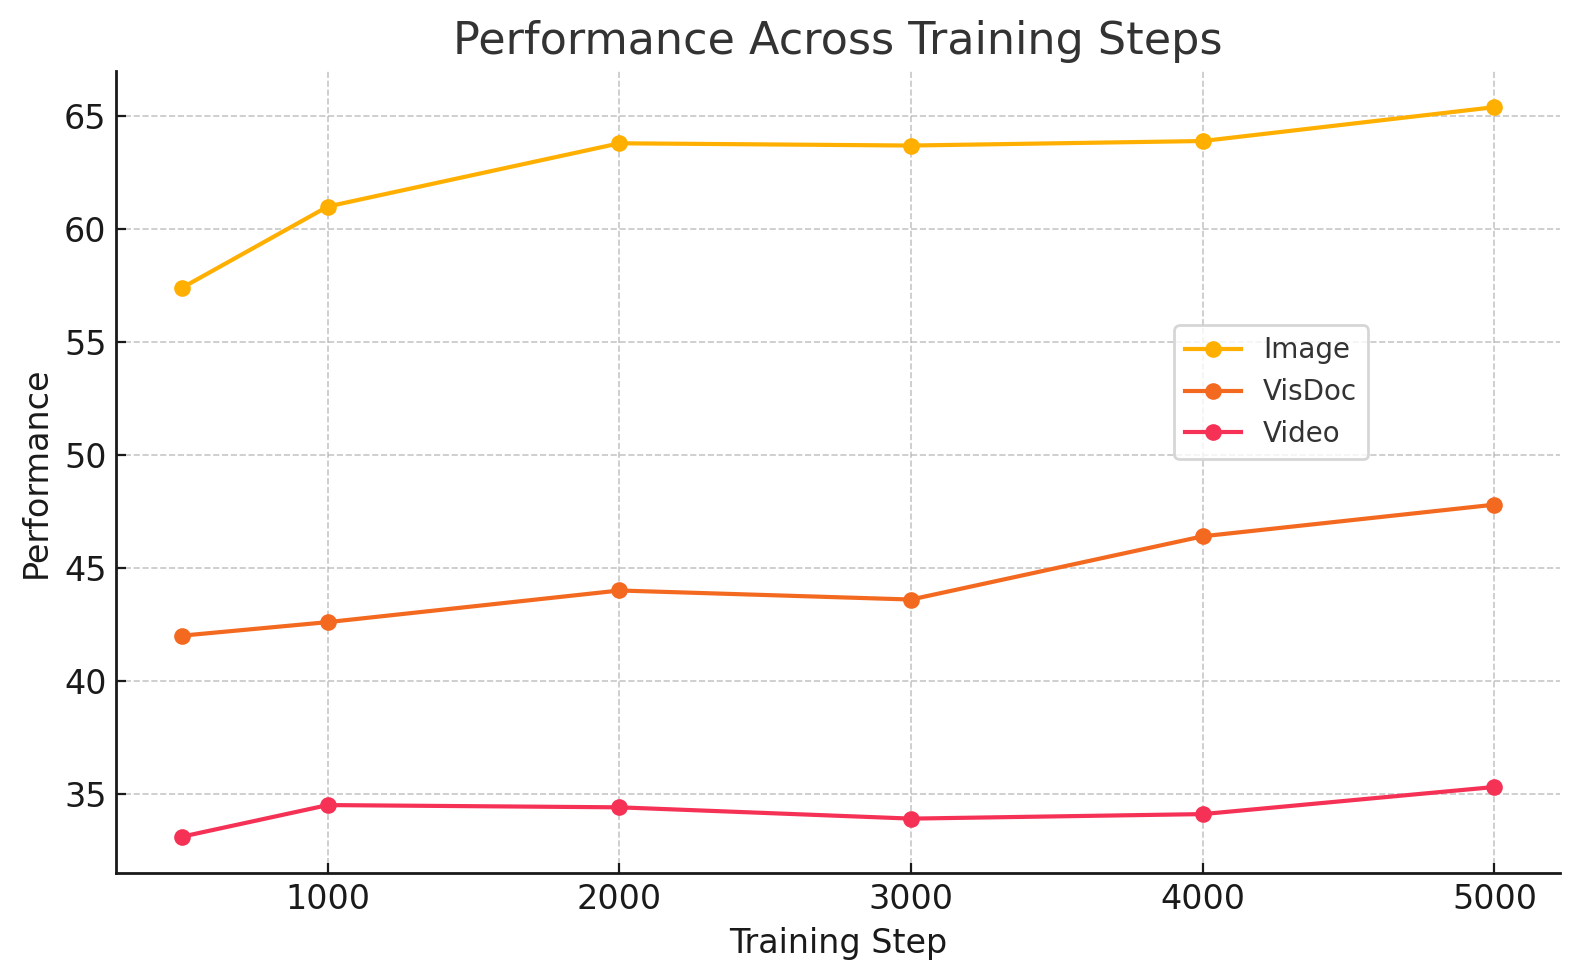
\includegraphics[width=0.75\textwidth]{figures/training_steps.png} % or .png
%     \caption{Performance across training steps for different modalities.}
%     \label{fig:training_steps}
% \end{figure}


\begin{figure}[ht]
    \centering
    \begin{subfigure}[t]{0.27\textwidth}
        \centering
        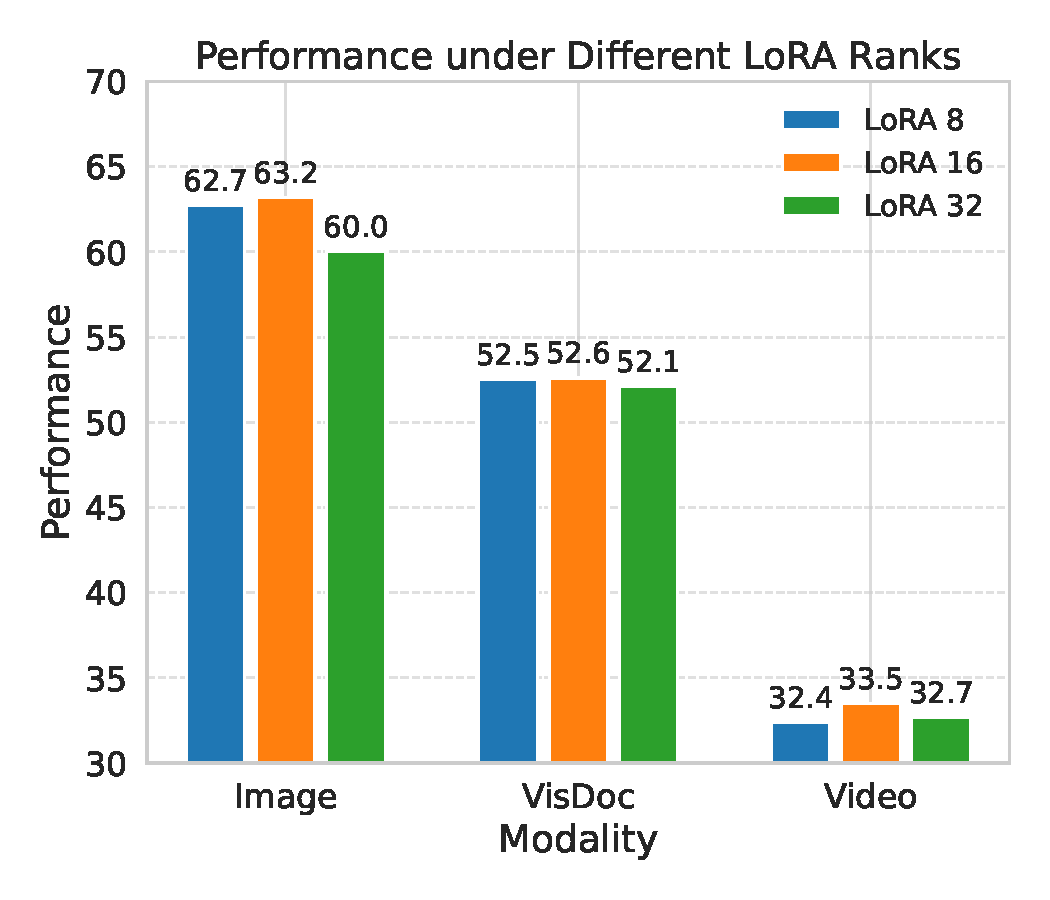
\includegraphics[width=\textwidth]{figures/lora_rank_comparison.pdf}
        % \caption{Performance across LoRA ranks for different modalities.}
        \label{fig:lora_ranks}
    \end{subfigure}
    \hfill
    \begin{subfigure}[t]{0.71\textwidth}
        \centering
        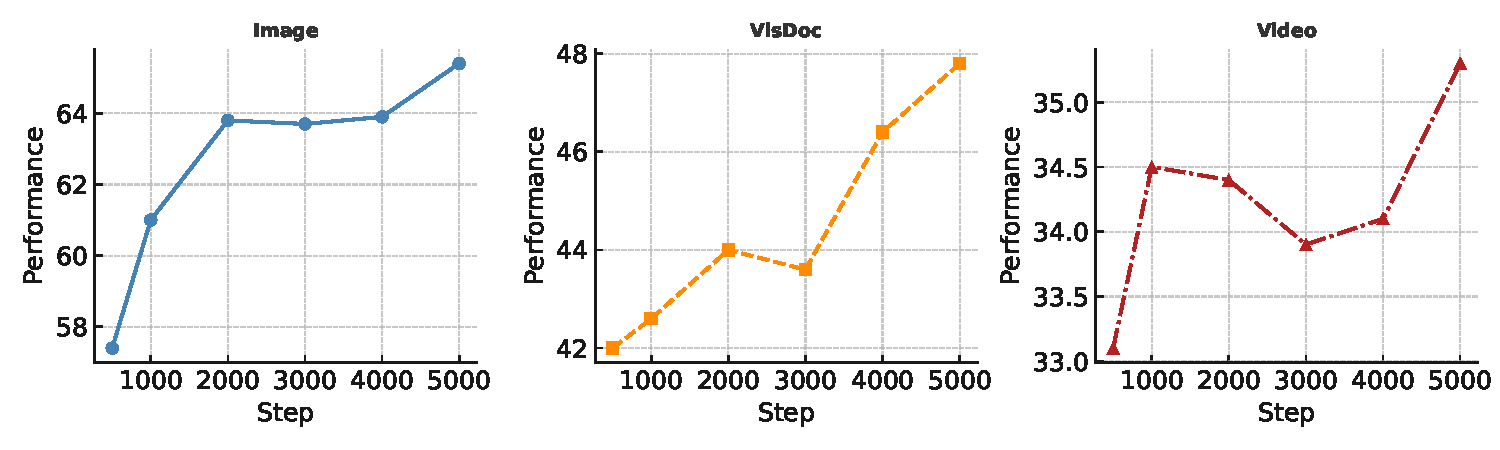
\includegraphics[width=\textwidth]{figures/training_step_per_modality.pdf}
        % \caption{Performance across training steps for different modalities.}
        \label{fig:training_steps}
    \end{subfigure}

    \caption{The left figure shows performance across LoRA ranks for different modalities, while the right figure illustrates performance trends across training steps.}
    
    % \semih{1. It is better to combine the 3 separate STEPs plots into a single one just like the bar plot on the left?} Rui: the initial figure is merged, but the layout looks too slim and the change was not very noticeable
    % \semih{2. Make the x-axis="Training Steps"}
    \label{fig:multi_modality}
\end{figure}


